In this chapter, we study existing techniques related to code generators testing as well as compilers auto-tuning techniques.
Section 2.1 provides a survey of the most used compiler auto-tuning techniques to construct the best set of optimization options. In Section 2.2, we review existing techniques for code generators testing. Section 2.3 discusses the limitations of the state of the art.
\section{Compilers}
The compiler is a very essential software component in software engineering, responsible for translating user'source code written in general purpose languages into machine code.


Compilers are typically platform dependent and translate programs written on the high-level language into the
assembly language or machine code of the targeted architecture. Produced assemblies.

Every high-level programming language (except strictly interpretive languages) comes with a compiler.

\section{Compiler optimizations}
High-level programming languages offer many abstract programming features such as functions, conditional statements and loops that facilitates software development. However, writing code in a high-level programming language may induce significant decrease in performance. Principally, software developers should write understandable, maintainable code without putting too much emphasizes on the performance for example. 
For this reason, compilers attempt generally to automatically optimize the code to improve its performance.

They can transform loops, conditional statements, and recursive functions; eliminate whole blocks of code; and take advantage of the target instruction set architecture (ISA) to make the code fast and compact. It’s much better to focus on writing understandable code, than making manual optimizations that result in cryptic, hard-to-maintain code. In fact, manually optimizing the code might prevent the compiler from performing additional or more efficient optimizations.

Rather than manually optimizing code, you should consider aspects of your design, such as using faster algorithms, incorporating thread-level parallelism and using framework-specific features (such as using move constructors).

Compilers become quite sophisticated in doing so nowadays. In fact, creating compiler optimizations for a new microprocessor is a hard and time-consuming work. 
Compilers are constantly improving in terms of the techniques they use to optimize the code. However, they’re not perfect.

\section{Iterative compilation}
Iterative compilation consists on applying software engineering techniques to produce better and more optimized programs by compiling multiple versions of each of them using different optimizations settings. After running these versions on specific hardware machines, the key objective of iterative compilation is to find the best optimizing sequence that lead to the fastest and better code machine code. 
Our work is related to iterative compilation research field.
The basic idea of iterative compilation is to explore the compiler optimization space by measuring the impact of optimizations on software performance.
Several research efforts have investigated this optimization problem using search-based techniques (SBSE) to guide the search towards relevant optimizations regrading performance, energy consumption, code size, compilation time, etc. Experimental results have been usually compared to standard compiler optimization levels.  
The vast majority of the work on iterative compilation focuses on increasing the speedup of new optimized code compared to standard compiler optimization levels~\cite{almagor2004finding,hoste2008cole,pan2006fast,pallister2015identifying,chen2012deconstructing,martins2014exploration,lin2008automatic,martinez2014multi}.
It has been proven that optimizations are highly dependent on target platform and input program. 
Compared to our proposal, none of the previous work has studied the impact of compiler optimizations on resource usage. In this work, we rather focus on compiler optimizations related to resource consumption, while bearing in mind the performance improvement.

\subsection{Implementation of Iterative Compilation System}
\begin{figure}[h]
	\center
	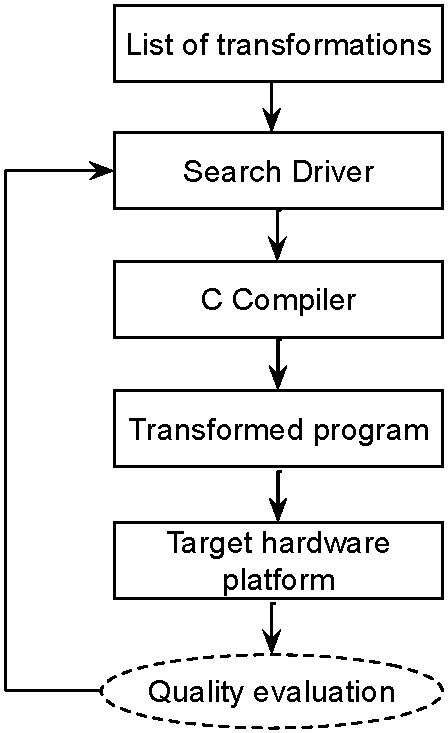
\includegraphics[scale=0.65]{SOTA/fig/iterative_compilation.pdf}
	\caption{Overview of the iterative compilation process}
	\label{fig:iterative_compilation}
\end{figure}
The implementation of iterative compilation consists mainly on applying a series of steps to enhance the quality of generated code. Figure~\ref{fig:iterative_compilation} shows a general overview of the principal steps needed to ensure the implementation of the iterative compilation system.
\begin{itemize}
	\item List of transformations
	\item Search driver
	\item C Compiler
	\item Transformed program
	\item Target hardware platform
	\item Quality evaluation
	
\end{itemize}
The first is to define the list of transformations that are provided by the target compiler. This list define the different optimizations that the compiler can apply to enhance the software quality. 
\subsubsection{Search-based techniques}
\paragraph{Genetic algorithm}
\paragraph{Multi-objective algorithm}
\section{Functional requirements}
Compilers verification and validation rely on the use of test suites to check the functional correctness of transformed code. There are sever

\section{Testing compilers}

Novelty Search has never been applied in the field of iterative compilation. Our work presents the first attempt to introduce diversity in the compiler optimization problem. 
The idea of NS has been introduced by Lehman et al.~\cite{lehman2008exploiting}. It has been often evaluated in deceptive tasks and especially applied to evolutionary robotics~\cite{risi2010evolving,krvcah2012solving} (in the context of neuroevolution). 
NS can be easily adapted to different research fields. In a previous work~\cite{boussaa2015novelty}, we have adapted the general idea of NS to the test data generation problem where novelty score was calculated as the Manhattan distance between the different vectors representing the test data. The evaluation metric of generated test suites is the structural coverage of code.
In this paper, the evaluation metric represents the non-functional improvements and we are calculating the novelty score as the symmetric difference between optimization sequences. 

For multi-objective optimizations, we are not the first to address this problem. New approaches have emerged recently to find trade-offs between non-functional properties~\cite{hoste2008cole,martinez2014multi,lokuciejewski2010multi}. Hoste et al.~\cite{hoste2008cole}, which is the most related work to our proposal, propose COLE, an automated tool for optimization generation using a multi-objective approach namely SPEA2. In their work, they try to find Pareto optimal optimization levels that present a trade-off between execution and compilation time of generated code. Their experimental results show that the obtained optimization sequences perform better than standard GCC optimization levels. NOTICE provides also a fully automated approach to extract non-functional properties. However, NOTICE differs from COLE because first, our proposed container-based infrastructure is more generic and can be adapted to other case studies (i.e., compilers, code generators, etc.). Second, we provide facilities to compiler users to extract resource usage metrics using our monitoring components. Finally, our empirical study investigates different trade-offs compared to previous work in iterative compilation.



%For code generators testing, Stuermer et al.~\cite{stuermer2007systematic} present a systematic test approach for model-based code generators. They investigate the impact of optimization rules for model-based code generation by comparing the output of the code execution with the output of the model execution. 
%If these outputs are equivalent, it is assumed that the code generator works as expected. 
%They evaluate the effectiveness of this approach by means of testing optimizations performed by the TargetLink code generator. 
%They have used Simulink as a simulation environment of models. 
%In our approach, we provide a component-based infrastructure to compare non-functional properties of generated code rather than functional ones. 


\section{Testing code generators}
Previous work on non-functional testing of code generators focuses on comparing, as oracle, the non-functional properties of hand-written code to automatically generated code~\cite{stepasyuk2015evaluating,richard2013efficient}. As an example, Strekelj et al.~\cite{vstrekelj2015performance} implemented a simple 2D game in both the Haxe programming language and the native environment and evaluated the difference in performance between the two versions of code. They showed that the generated code through Haxe has better performance than hand-written code. 

Cross-platform mobile development has been also part of the non-functional testing goals since many code generators are increasingly used in industry for automatic cross-platform development. In \cite{pazirandeh2015evaluation,hartmann2011cross}, authors compare the performance of a set of cross-platform code generators and presented the most efficient tools.

The container-based infrastructure has been also applied to the software testing, especially in the cloud~\cite{li2015rest}. Sun et al.~\cite{sun2016roar} present a tool to test, optimize, and automate cloud resource allocation decisions to meet QoS goals for web applications. Their infrastructure relies on Docker to gather informations about the resource usage of deployed web servers. 

Most of the previous work on code generators testing focuses on checking the correct functional behavior of generated code. Stuermer et al.~\cite{stuermer2007systematic} present a systematic test approach for model-based code generators. They investigate the impact of optimization rules for model-based code generation by comparing the output of the code execution with the output of the model execution. 
If these outputs are equivalent, it is assumed that the code generator works as expected. 
They evaluate the effectiveness of this approach by means of testing optimizations performed by the TargetLink code generator. 
They have used Simulink as a simulation environment of models. 
In \cite{jorges2014back}, authors presented a testing approach of the Genesys code generator framework which tests the translation performed by a code generator from a semantic perspective rather than just checking for syntactic correctness of the generation result.

Compared to our proposal, none of the previous work has provided an automatic approach for testing and monitoring the generated code in terms of non-functional properties. 

\iffalse
Our work is related to iterative compilation research field.
The basic idea of iterative compilation is to explore the compiler optimization space by measuring the impact of optimizations on software performance.
Several research efforts have investigated this optimization problem to catch relevant optimizations regrading performance, energy or code size improvements over standard optimization sequences~\cite{almagor2004finding,hoste2008cole,pan2006fast,zhong2009tuning,pallister2015identifying,chen2012deconstructing,sandran2012genetic,martins2014exploration,fursin2008milepost,lin2008automatic,schulte2014post}. 
The vast majority of the work on iterative compilation focuses on increasing the speedup of new optimized code compared to standard optimizations. 
It has been proven that optimizations are highly dependent on target platform and input program. Compared to our proposal, we rather focus on comparing the resource consumption of optimized code.

Novelty Search has never been applied in the filed of iterative compilation. Our work presents the first attempt to introduce diversity in optimization sequences generation. The idea of NS has been introduced by Lehman et al.~\cite{lehman2008exploiting}. It has been often evaluated in deceptive tasks and especially applied to evolutionary robotics~\cite{risi2010evolving,krvcah2012solving} (in the context of neuroevolution). 
NS can easily be adapted to different research fields. In a previous work~\cite{boussaa2015novelty}, NS has been adapted for test data generation where novelty score was calculated as the Manhattan distance between the different vectors representing test data.
In our NS adaptation, we are measuring the novelty score using the systematic difference between optimization sequences of GCC.

For code generators testing, Stuermer \etal present a systematic test approach for model-based code generators~\cite{stuermer2007systematic}. They investigate the impact of optimization rules for model-based code generation by comparing the output of the code execution with the output of the model execution. 
If these outputs are equivalent, it is assumed that the code generator works as expected. 
They evaluate the effectiveness of this approach by means of testing optimizations performed by the TargetLink code generator. 
They have used Simulink as a simulation environment of models. 
In our approach, we provide a component-based infrastructure to compare non-functional properties of generated code rather than functional ones. 
\fi
